\documentclass[10pt,a4paper]{report}
\usepackage[utf8]{inputenc}  
\usepackage[T1]{fontenc}      
\usepackage[francais]{babel}
\usepackage{amsmath}
\usepackage{amsfonts}
\usepackage{amssymb}
\usepackage{graphicx}
\usepackage{hyperref}
\usepackage{caption}
\author{Thomas Citharel}
\title{Rapport de stage}
\begin{document}
	\maketitle
	\tableofcontents
	\chapter*{Introduction}
	J'aime les gaufres
	\chapter{Présentation du stage}
	\section{Présentation de la structure d'accueil}
	J'ai effectué mon stage au sein de l'association \textbf{Framasoft} dont les buts sont la promotion, la diffusion et le développement de logiciels libres, de services libres en ligne et de la culture libre. Framasoft (pour \textbf{fra}nçais et \textbf{ma}thématiques) a commencé en 2001 comme un site annuaire de logiciels libres avant de devenir une association Loi 1901 en 2004. Depuis l'annuaire de logiciels libres qui n'a cessé de se remplir, on peut noter les projets suivants proposés par l'association :
	\begin{itemize}
		\item la \textbf{Framakey}, clé USB contenant une sélection de logiciels libres à utiliser directement sous Windows, Linux ou MacOS X ;
		\item les \textbf{Framabooks}, une collections d'ouvrages (Romans, BD, Manuels) diffusés sous différentes licences libres ;
		\item le \textbf{Framablog}, qui parle de logiciels et de culture libre en lien avec l'actualité mais propose également des traductions d'articles dans des langues étrangères.
	\end{itemize}
	
	En octobre 2014, la campagne \href{https://degooglisons-internet.org/}{\textbf{\textit{Dégooglisons} Internet}} est lancée dans le but de montrer au public que des solutions sont possibles face aux services proposés par les \textit{géants du net} (aussi nommés \textit{GAFAM} pour Google, Amazon, Facebook, Apple et Microsoft).
	
	Depuis le lancement de la campagne Framasoft a déjà ouvert une vingtaine de services en ligne et il en est prévu davantage d'ici la fin de la campagne en 2017.
	
	Framasoft utilise donc des applications web libres existantes ou développe ses propres alternatives pour proposer à des personnes non-techniques des services viables.
	
	Ainsi, l'association a fait développer des solutions spécialement pour proposer \textbf{Framapic} (hébergement d'images : alternative à Imgur, Flickr), \textbf{Framalink} (raccourcisseur d'url : alternative à bit.ly) et \textbf{Framadrop} (service de transfert de fichiers : alternative à WeTransfer).
	
	\section{Présentation du projet}
	
	Pour ma part, je devais développer une alternative à Google Calendar nommée \textbf{Framagenda}. En accord avec mon maître de stage, cette alternative s'est basée sur le logiciel libre ownCloud dont la fonctionnalité principale est le service d'hébergement de fichiers (en alternative à DropBox) mais qui propose de nombreuses applications tierces dont une faisant office de calendrier.
	
	\subsection{Background technique}
	ownCloud est une application web libre écrite en PHP. Elle consiste en un cœur (dénommé par la suite comme \textit{core}) qui s'occupe essentiellement de la gestion des utilisateurs, de la gestion des fichiers, de la gestion des partages et de la fédération et propose des API aux applications tierces. Les applications (calendrier, contacts, prise de notes, lecteur de flux RSS) sont ainsi intégrées à ownCloud.
	
	Un serveur de calendrier doit suivre les standards CalDAV, qui est une extension du protocole WebDAV appliquée aux fichiers iCalendar. WebDAV est un protocole de gestion de fichiers sur serveurs distants conçu comme une extension du standard HTTP. \href{https://tools.ietf.org/html/rfc2445}{iCalendar} est un standard assez vieux (1998 !) qui décrit le format d'un fichier agenda.
	
	Dans notre cas, le serveur est géré avec le concours d'une librairie du nom de SabreDAV qui gère CalDAV, CardDAV (pour les contacts) et WebDAV. Cette librairie fonctionne avec un système de plugins nous permettant de l'adapter pour notre utilisation dans ownCloud.
	
	\subsection{Aie Aie Aie}
	
	Il est important de remarquer que les protocoles internet pour la gestion de calendrier souffrent de multiples défauts rendant la compatibilité entre serveurs de calendrier et clients plutôt bancale.
	
	Ainsi, c'est la société Apple qui est à la pointe des derniers standards dans son application \textit{iCal} (désormais nommée plus simplement \textit{Calendar}). N'ayant pas de machine Apple, je n'ai pu profiter de ce logiciel pour mes tests. De plus, le protocole CalDAV utilisé est pour le moins critiqué.
	
	Quelques mois avant que mon stage débute, deux événements ont eu lieu. D'une part, ownCloud a sorti une version 9.0 qui a transféré le module DAV (serveur responsable du calendrier et des contacts) dans le \textit{core} et l'application Calendar a été refaite complètement quasiment intégralement en javascript à l'aide du framework AngularJS.
	
	D'autre part, la communauté et l'entreprise derrière ownCloud se sont pris le chignon, aboutissant à la création d'un \textit{fork} du nom de NextCloud. Heureusement, je me suis aperçu que les deux projets continuaient à communiquer et à échanger du code.
	
	\subsection{Le deal}
	Je devais effectuer les tâches suivantes :
	
	\subsubsection{Permettre de rendre un calendrier public et l'afficher publiquement sans être enregistré sur l'instance ownCloud.}
	
	La première tâche était la mission principale. Elle est liée premièrement à l'implémentation du protocole de publication d'un calendrier tel que défini par Apple à travers un plugin spécialisé dans le cœur d'ownCloud. D'autre part, il nous faut également une interface utilisateur dans l'application Calendrier qui permette de publier et dé-publier un calendrier. Enfin, il était nécessaire de proposer une vue « publique » accessible à tous sans être enregistré pour les calendriers publiés.
	
	\begin{figure}
		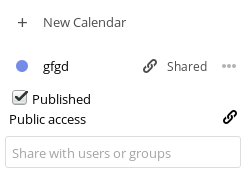
\includegraphics[width=0.5\paperwidth]{images/fonctionnalitepublie.png}
		\caption*{Un calendrier publié}
		\label{normal_case}
	\end{figure}

	
	\begin{figure}[ht]
		\centering
		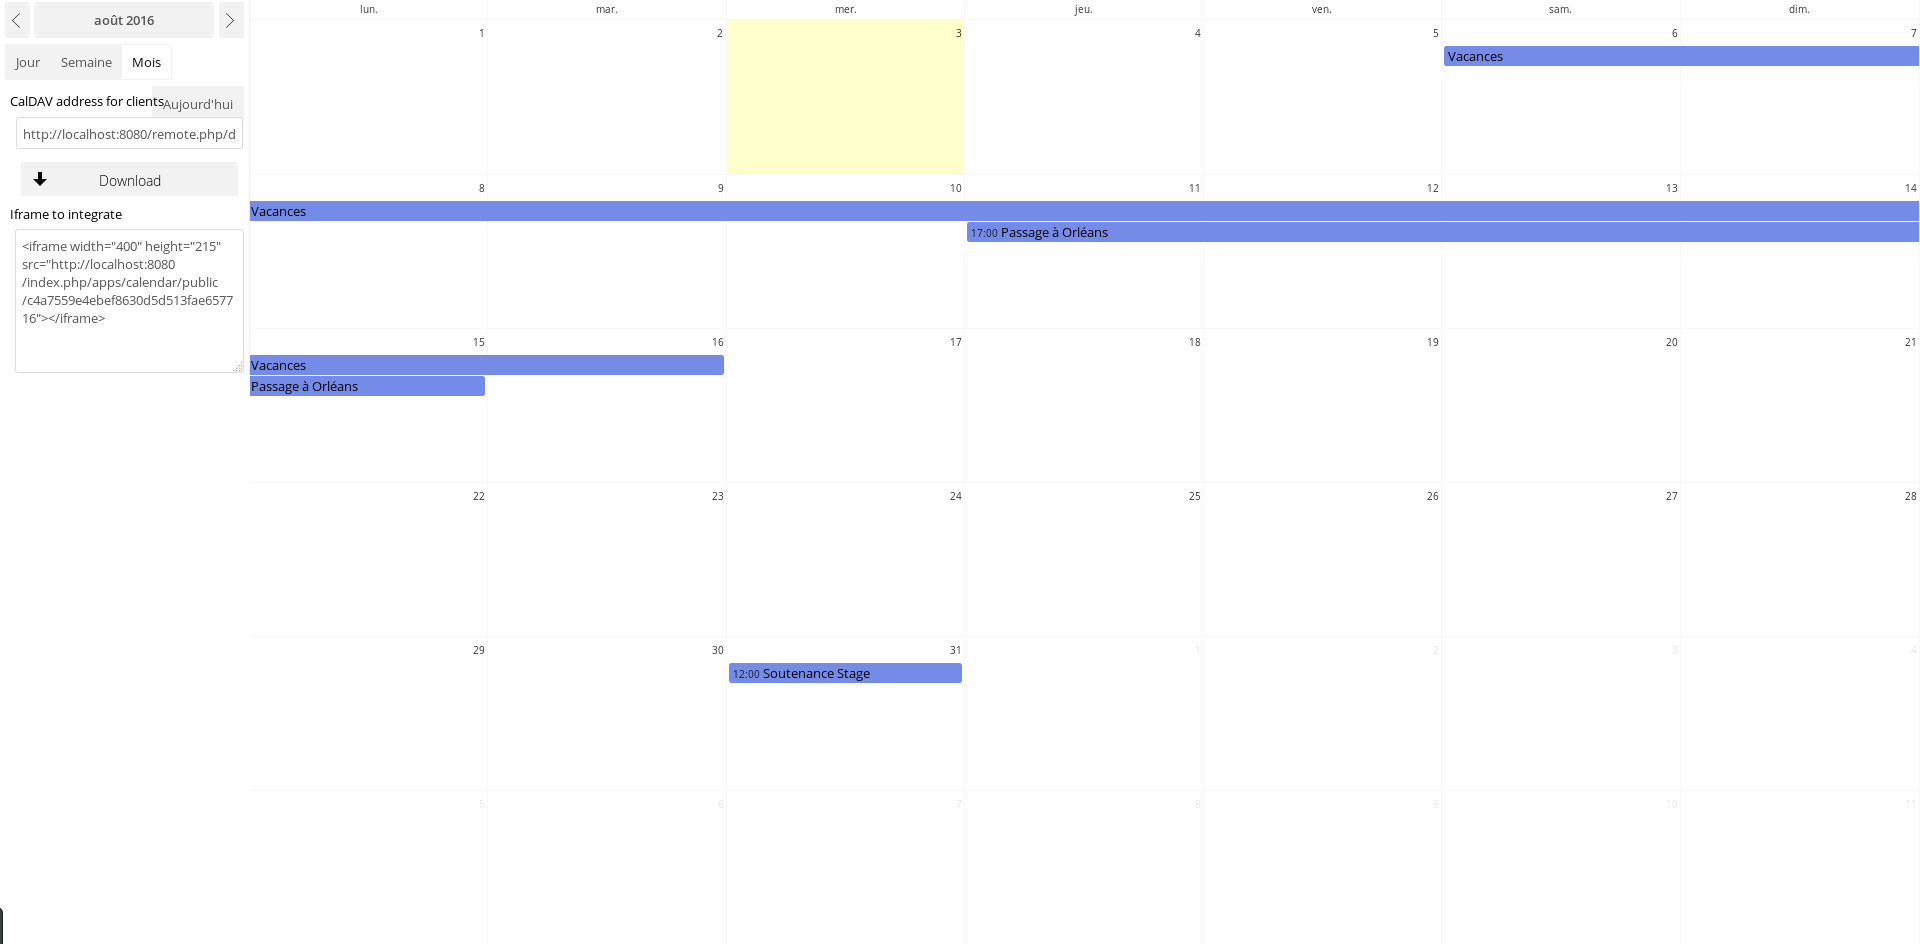
\includegraphics[width=1\textwidth]{images/calendrier-vue-publique.png}
		\caption*{Vue publique d'un calendrier}
		\label{normal_case}
	\end{figure}

	
	\subsubsection{ Permettre d'afficher ce calendrier public à l'intérieur d'une \textit{iframe} lui permettant d'être intégré sur des sites tiers ou des blogs.}La seconde tâche était assez simple et consistait surtout à configurer l'application correctement pour autoriser l'intégration à l'intérieur de sites tiers, et de rendre son apparence acceptable.
	
	\begin{figure}
		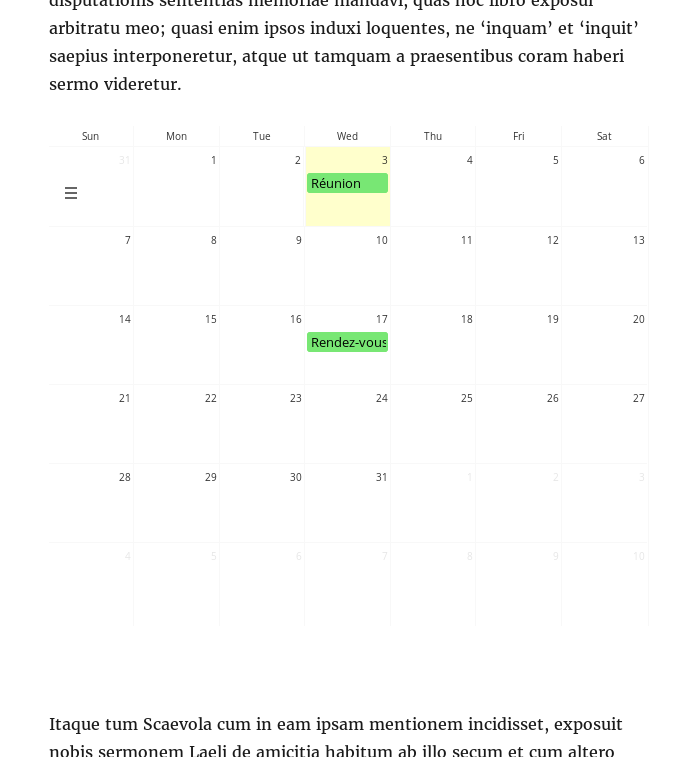
\includegraphics[width=0.5\paperwidth]{images/integration_wordpress}
		\caption*{Intégration d'un calendrier public dans une page Wordpress}
		\label{normal_case}
	\end{figure}
	
	\subsubsection{Permettre de s'abonner à des calendriers, c'est à dire de visualiser des calendriers dans l'application qui proviennent d'une source publique sur internet.}
	
	\begin{figure}[ht]
		\centering
		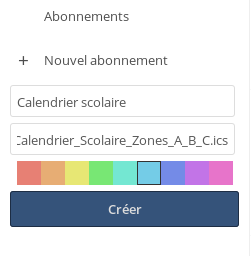
\includegraphics[width=0.30\textwidth]{images/creation_abonnement.png}
		\caption*{Formulaire pour ajouter un calendrier public}
		\label{normal_case}
	\end{figure}
	
	La troisième tâche consistait à pourvoir une fonctionnalité d'abonnement à des calendriers dans l'application Calendrier d'ownCloud. En effet, l'implémentation des abonnements selon le standard CalDAV était déjà réalisée dans le cœur d'ownCloud, il suffisait de réaliser les bons appels et de gérer les fichiers distants.
	
	\chapter{History}
	La première semaine de mon stage a été dédiée à l'étude du fonctionnement du cœur d'ownCloud et l'intégration avec SabreDAV. J'ai dû également rechercher beaucoup d'informations sur les standards de CalDAV (ainsi que ce qui n'est pas standardisé !) car la synchronisation devait fonctionner à partir des clients existants.
	
	D'autre part, j'ai également dû lire beaucoup du code de l'application Calendrier, car elle est développée à l'aide du Framework AngularJS qui n'est pas une technologie que je maîtrisais.
\end{document}